\chapter{Large Language Models}\label{ch:techOverview}

Creating machines with human-like language understanding has been a subject of research since the 1950s.
\gls{natural-language}s are highly complex and pose a difficult challenge to computers.
% ambiguous: ~\autocite{quadarLM2020}
\gls{lm} is an approach to make machines read, write and communicate like humans~\autocite{zhao2023survey}.

The main idea of \gls{lm} is to estimate probability distributions over units of texts, e.g.\ words~\autocite{de2015survey}.
Assuming that the occurrence of a word depends on previous words, i.e.\ the context, the probability of that word being next in a sentence can be modeled with a conditional probability~\autocite{jozefowicz2016exploring}.
\[
    P(w_n | w_1, \dots , w_{n-1})
\]
% TODO: quelle finden vielleicht
The ability to estimate the probability distributions over words makes it possible to predict the next word for a given sequence.
In this way, language models can be applied in many \gls{nlp} tasks like speech recognition, machine translation and text summarization~\autocite{jozefowicz2016exploring}.
By simply predicting the next word, language models can hold human-like conversations, which makes it appear as if they understand natural language.
% How would translation look like?
% TODO: Other approaches like BERT Masked language Modeling
%Other approaches to \gls{lm} mask parts of sentences and use all surrounding language units to predict the missing

There are different techniques to model these probabilities of word sequences.
In the 1990s, \glspl{slm} found widespread use.
The models often assume that the distribution of a word only depends on a fixed length of previous words.
\enquote{$n$-grams models} are \glspl{slm} that use the previous $n$ words to calculate the probability distribution of the next word.
Based on a training corpus, tables of conditional probabilities are created.
The probabilities are approximated by counting occurrences of $n$-grams.
If the previous word is \enquote{thank}, the probability that the next word is \enquote{you} could be estimated as follows~\autocite{quadarLM2020}
\[
    P(\text{you} | \text{thank}) = \frac{P(\text{thank you})}{P(\text{thank})} \approx \frac{count(\text{thank you})}{count(\text{thank})}
\]
In recent years, research has been focused on the more flexible \glspl{nlm}~\autocite{quadarLM2020}.
This approach uses \glspl{dnn} to estimate the needed probability distributions.
\glspl{nlm} are much better at taking long-range depencies in text into account than \glspl{slm}~\autocite{Hadi_2023}.
\glspl{dnn} excel at extracting complex features from text and finding meaningful representations for words.
These representations (often called embeddings) lie in a vector space of real vectors where similar words are close to each other in a mathematical sense~\autocite{quadarLM2020}.
In \glspl{nlm} the prediction function is usually built on top of these embeddings.
The intermediate step of learning effective features and representing them in embeddings has the benefit that those embeddings can be reused for other tasks.
The early 2010s saw the rise of \glspl{dnn} that were specifically designed to create powerful word embeddings~\autocite{zhao2023survey}.
These embeddings were static, meaning the network would assign each word exactly one embedding, disregarding polysemy of words~\autocite{Liu_2020}.
Embeddings of popular solutions like \enquote{word2vec} proved to be very useful in various \gls{nlp}-Tasks.

Following research focused on incorporating context into word embeddings, i.e.\ assigning a different vector representation to a word depending on the surrounding words.
ELMo, BERT and GPT are well-known models that managed to do so.
These context-aware language models are trained on large unlabeled corpora of text data.
During training, the models learn to solve pre-training tasks that are specifically designed for the language model to gain essential language understanding.
They are often put into their own class of language models, the so-called \glspl{plm}.
\glspl{plm} set new standards in solutions of many \gls{nlp}-tasks.
They learn general-purpose features that can be effectively used by fine-tuning the models on downstream tasks, e.g.\ machine translation, text summarization or \gls{ats}.
The process of using a \gls{plm} as a base model to fine-tune it for a specific task has become a commonly used pattern in \gls{lm}~\autocite{zhao2023survey}.

The availability of huge datasets and powerful computing devices led to another evolution in \gls{lm}.
\glspl{llm} are \glspl{plm} that are scaled in model size.
They are usually based on the popular transformer architecture~\autocite{Hadi_2023} and consist of billions of parameters.
Research found that using larger models with more extensive pre-training on larger datasets greatly improves performance~\autocite{Raiaan2024ARO}.
\glspl{llm} even show unexpected abilities (called emergent abilities) that could not be observed in smaller models, e.g.\ reasoning and solving complex tasks without fine-tuning~\autocite{zhao2023survey}.
They are capable of \enquote{in-context learning} meaning they can perform tasks given only instructions and a few examples without the need of updating model parameters~\autocite{bhatia2023tart}.
ChatGPT is an example of a popular \gls{LLM} with amazing conversation and task solving abilities~\autocite{zhao2023survey}.

While \glspl{llm} produce impressive results with \enquote{in-context learning} they are usually still outperformed by fine-tuned language models in specific tasks~\autocite{bhatia2023tart}.
In the context of German \gls{ats} this is supported by the results of~\textcite{deilen2023using} who find that ChatGPT can only create very rudimentary simplifications.

The course of action for this thesis is to use pre-trained base models to fine-tune them on the task of \gls{ats}.
Due to hardware limitations, only \glspl{plm} with up to 13 billion parameters come into question.
In the following sections the underlying workings of \glspl{nlm}, \glspl{plm} and \glspl{llm} will be explained.

% TODO
\begin{figure}
    \centering
    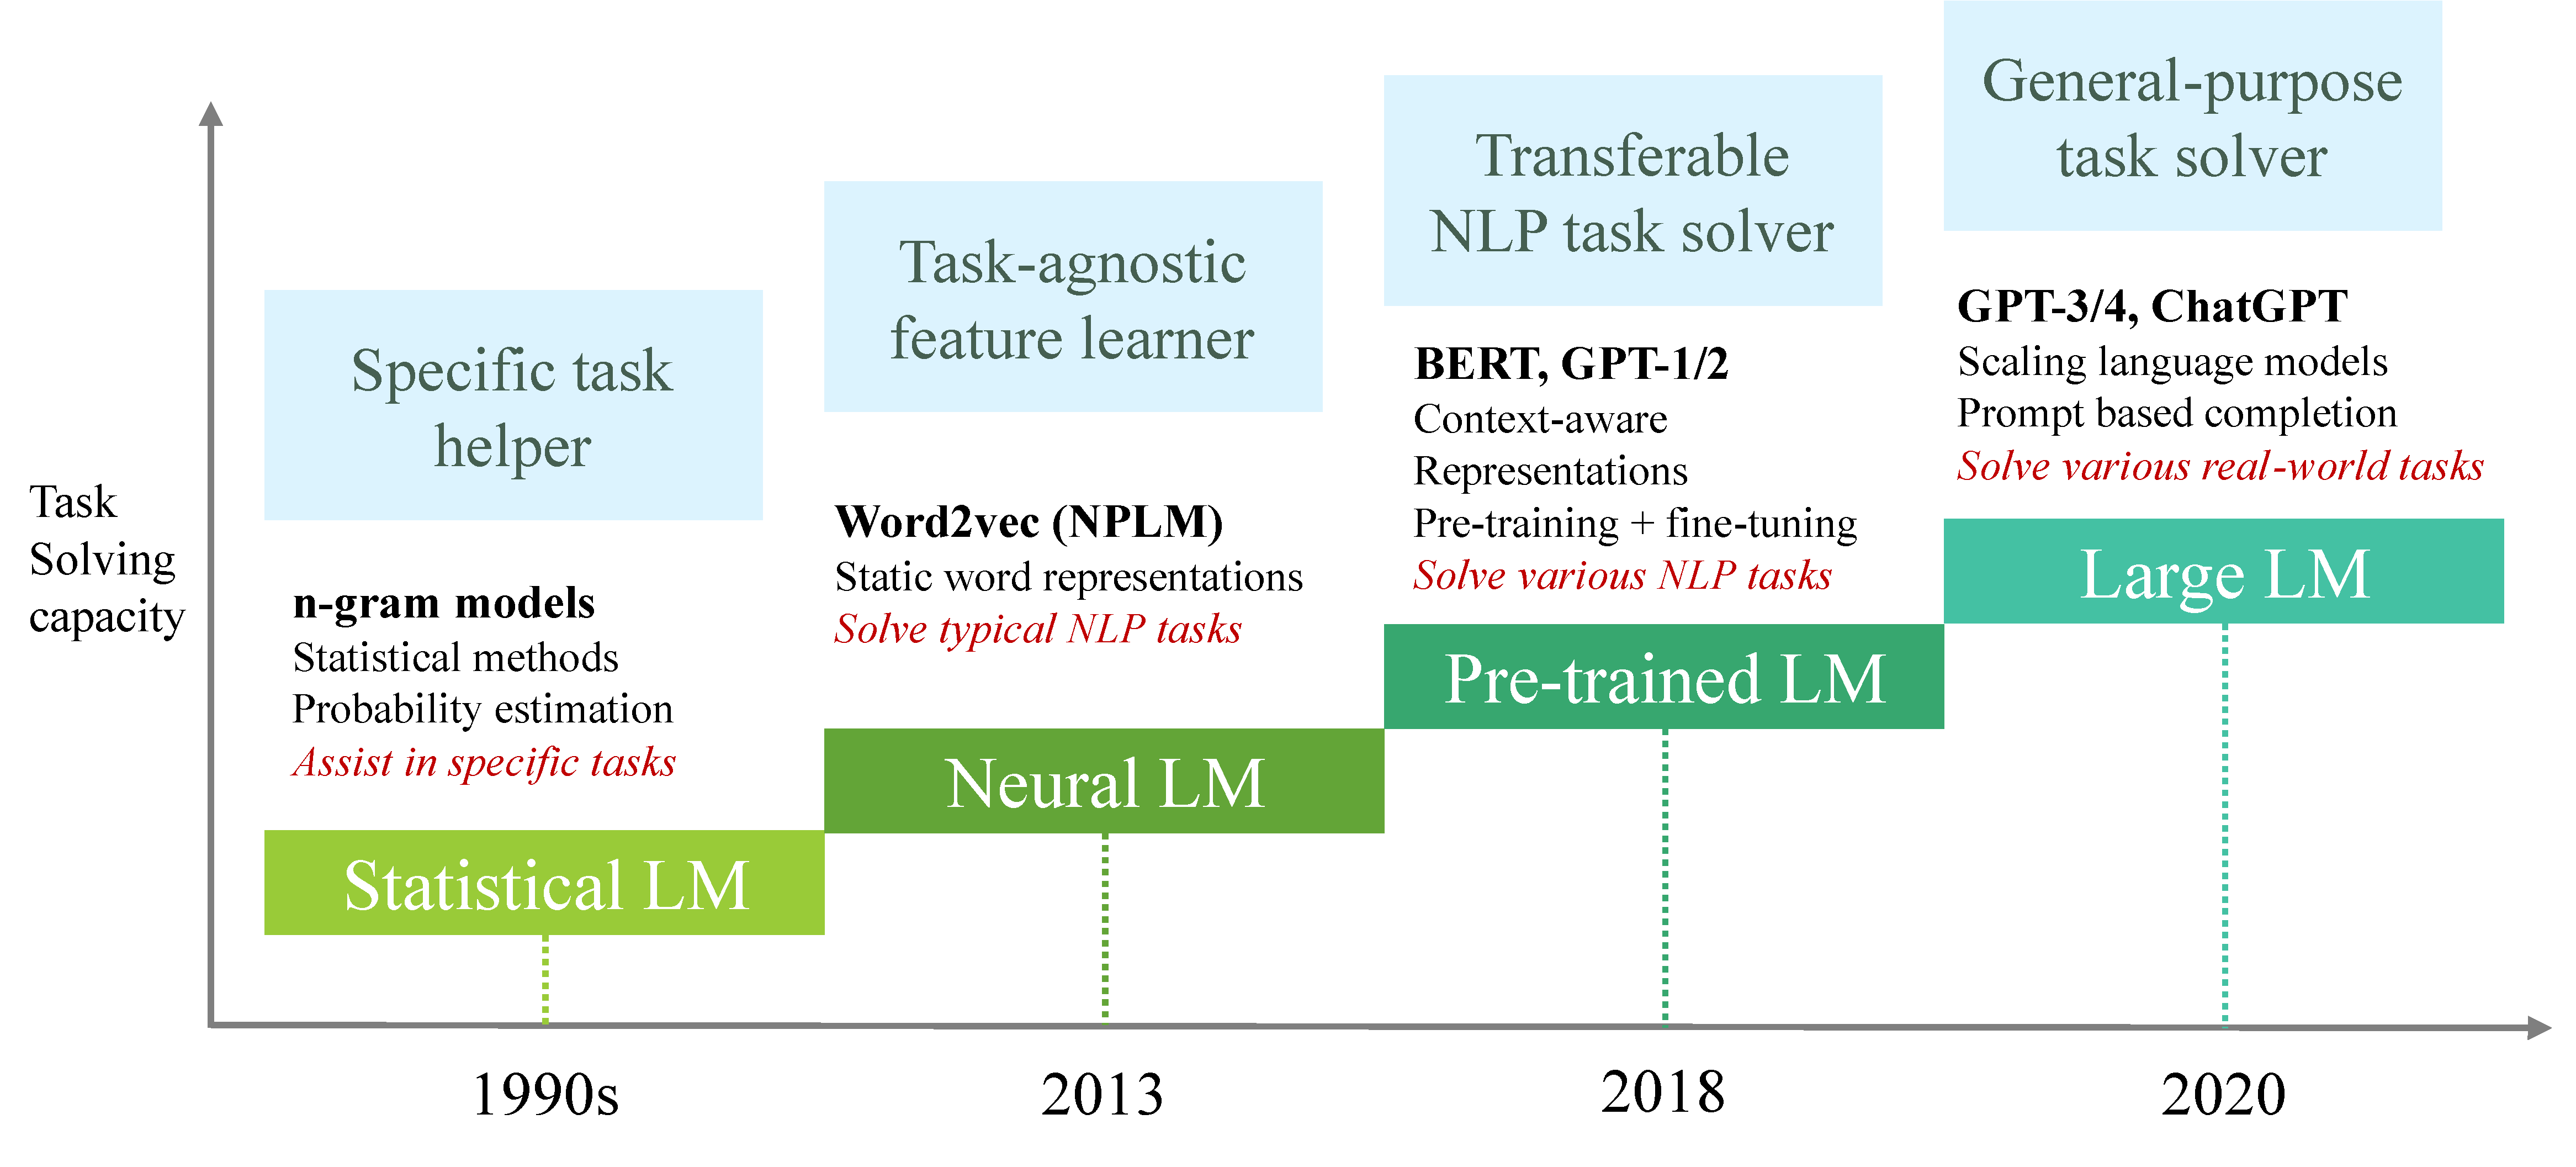
\includegraphics[width=\linewidth]{images/languagemodels}
    \caption[TODO.]{TODO~\autocite{zhao2023survey}}
    \label{fig:language-models}
\end{figure}

%With the introduction of the transformer architecture in 2017~\autocite{vaswani2023attention}
%task-agnostic representations -> less human feature engineering~\autocite{zhao2023survey}

%from~\autocite{zhao2023survey}:
%language modeling to task solving

%from ~\autocite{Raiaan2024ARO}:
%pre-training on large corpora from the web -> learning complicated patterns and language subtleties
%fine-tuning on downstream tasks gives state-of-the-art performance
%"comprehend, produce, forecast human language"

%From ~\autocite{Hadi_2023}:
%during pre-training: models see diverse texts and learn grammar, facts, reasoning

\clearpage


\section{Deep Learning}\label{sec:deep-learning}
As previously mentioned, \glspl{dnn} are the underlying technology for modern language models.
\glspl{dnn} belong to the field \enquote{Deep Learning} which is a specific type of \gls{ml}.
The term \acrlong{ml} describes different computational methods that can learn to perform different tasks from experiencing data~\autocite{Goodfellow-et-al-2016}.

A typical application for \gls{ml} is to learn a task that can be represented by a mapping:
\[
    f: \mathcal{X} \rightarrow \mathcal{Y}
\]
The \textit{input space} $\mathcal{X}$ is the set of all possible \textit{examples}.
Each example is mapped to a \textit{label} or \textit{target value} from the \textit{target space} $\mathcal{Y}$.
Input spaces often consist of real vectors $\boldsymbol{x} \in \mathbb{R}^n$.
The entries $x_i$ of an example vector are called \textit{features}.
Target spaces vary depending on the specific task.
Typical are subsets of natural numbers for \textit{classifications} or real numbers (e.g.\ for \textit{regression}).

For classification tasks, the learned function assigns an integer representing a category to each possible input example.
A common use case for this is the categorization of images.
An automatic image classifier $f:\mathbb{R}^n \rightarrow \{1,\dots,k\}$ receives an image (usually in the form of a real vector) and outputs a numerical value that symbolizes the content of that image e.g.\ a person, an object or an animal.

\gls{ml} offers a broad range of methods to find functions that can model complex behavior.
They incorporate many elements from different fields like linear algebra, probability theory, numerical optimization and information theory~\autocite{Goodfellow-et-al-2016}.
\gls{ml} has been successfully applied to numerous problems from different domains, including text classification, \gls{nlp}, speech processing applications, computer vision and computational biology applications.
\gls{ml}-approaches are usually categorized into the different learning scenarios \textit{supervised learning}, \textit{unsupervised learning} and \textit{semi-supervised learning}.
These scenarios differ in the usage and type of available training data~\autocite{mohri2018foundations}.
Supervised learning is especially relevant for machine translation tasks like \gls{ats}.

\subsection{Supervised Learning}\label{subsec:supervised-learning}
In the setting of supervised learning, available training data consists of pairs of input examples with corresponding target values.
\[
    D = \{(x_1, y_1), \dots, (x_m, y_m)\}
\]
The general aim is to model the relation between the examples $x_i$ and the targets $y_i$.
For that, assumptions about the origin of the data have to be made.
It is commonly assumed that the pairs $(x_i, y_i)$ are sampled from an unknown probability distribution, i.e.\ they are realizations of random variables $Z_i = (X_i, Y_i)$ that take values in $\mathcal{X} \times \mathcal{Y}$.
The random variables $\{(X_1, Y_1), \dots ,(X_m, Y_m)\}$ are independently and identically distributed (i.i.d.) while $X_i$ and $Y_i$ are not necessarily independent~\autocite{gressmann2019probabilistic}.
In the context of \gls{ml} this is often denoted as $(X_i,Y_i) \sim P(X, Y)$ where $P(X, Y)$ signifies the joint probability distribution (e.g.\ \textcite{Goodfellow-et-al-2016}).

In the setting of \enquote{classical} supervised learning, the objective is to learn a deterministic prediction function $f: \mathcal{X} \rightarrow \mathcal{Y}$ that defines a mapping between examples and targets:
\[
    \, (X^*, Y^*) \sim P(X, Y): \quad  Y^* = f(X^*)
\]
To approximate this mapping, a set of potential prediction functions $\mathcal{H}$ is considered.
% TODO example
The learning algorithm consists of choosing the hypothesis $h \in \mathcal{H}$ that is closest to the unknown prediction function $f$, i.e.\ $h(X^*) \approx f(X^*) = Y^*$.
In order to quantify the mathematical distance between predictions, a \textit{loss function} (sometimes called \textit{cost function} or \textit{error function}) $L: \mathcal{Y} \times \mathcal{Y} \rightarrow \mathbb{R}$ is used.
If $\mathcal{Y} = \mathbb{R}$ (e.g.\ for a regression) the \textit{least squares loss} $L_{sq} (\hat{y}, y) = (\hat{y} - y)^2$ is common~\autocite{gressmann2019probabilistic}.
The ideal hypothesis $h^*$ minimizes the expected generalization error (sometimes called \textit{risk})
\[
    h^* = \underset{{h \in \mathcal{H}}}{\operatorname{argmin}} \, \mathbb{E}[L(h(X^*), Y^*)]
\]
Because the underlying data distribution $P(X, Y)$ is unknown, this optimization problem is not solvable.
Instead, the observed training data $D$ is used to minimize an approximation of the risk, i.e\ the \textit{empirical risk}:
\[
    \hat{h} = \underset{{h \in \mathcal{H}}}{\operatorname{argmin}} \, \frac{1}{m}\sum_{i=1}^{m} L(h(x_i), y_i)
\]
This approach may lead to \textit{overfitting}, meaning the determined hypothesis $\hat{h}$ accurately describes the training data $D$ but does not generalize well on unseen data.
There are several methods to prevent this like regulating the complexity and capacity of functions included in $\mathcal{H}$ or using a larger dataset with more training examples.
By setting aside a small subset of the training data as \textit{test data} which is not used in the optimization process, it is possible to estimate the generalization error.
This is again done with the empirical quantity specified above.
The estimate indicates how well the chosen hypothesis $\hat{h}$ performs on unseen data.

While learning a direct mapping from $\mathcal{X}$ to $\mathcal{Y}$ can be adequate to model some tasks, many supervised learning algorithms estimate a conditional probability distribution $P(Y | X)$ instead.
This way, the model can consider the \textit{aspect of uncertainty} that is present in many real world applications for \gls{ml}.
In this scenario, the desired prediction function maps input examples to a distribution over the target space $f: \mathcal{X} \rightarrow \operatorname{Distr}(\mathcal{Y})$.
To evaluate predictions, an appropriate loss function $L: \operatorname{Distr}(\mathcal{Y}) \times \mathcal{Y} \rightarrow \mathbb{R}$ is necessary.
For a classification task, the output distribution could be a categorical distribution over all class labels, i.e.\ a discrete distribution that for a given example $x$ assigns each class a probability signifying a degree of belief~\autocite{Goodfellow-et-al-2016}.
This type of prediction function can easily be modified to mimic the behavior of the \enquote{classical} prediction function:
\[
    g(x) =\underset{y \in \mathcal{Y}}{\operatorname{argmax}} [f(x)](y) \approx \underset{y \in \mathcal{Y}}{\operatorname{argmax}} P(Y=y|X=x)
\]

\subsection{Learning from Data (Gradient Descent)}\label{subsec:learning-from-data}
Depending on the type of assumed hypothesis functions, different methods from the field of \enquote{mathematical optimization} can be used to minimize the empirical risk.
It is typical to consider a set of functions $\{h(\,\cdot\, ; \boldsymbol{\theta}) \mid \boldsymbol{\theta} \in \Theta \}$ as the hypothesis space $\mathcal{H}$ where $\boldsymbol{\theta}$ represents free, learnable parameters that can be adjusted so the prediction function $h$ can accurately fit the data $D$.
The parameter space $\Theta$ is often chosen as $\mathbb{R}^n$ meaning the function is parameterized by a vector of real numbers.
A simple example for such a set of functions is the linear combination $h(\boldsymbol{x}, \boldsymbol{\theta}) = x_1\theta_1 + \dots + x_n\theta_n$.

The empirical risk can then be formulated as a function $\mathcal{L}: \Theta \rightarrow \mathbb{R}$:
\[
    \mathcal{L}(\boldsymbol{\theta}) = \frac{1}{m}\sum_{i=1}^{m} L(h(x_i, \boldsymbol{\theta}), y_i)
\]
Finding the hypothesis $\hat{h}$ that most accurately describes the training data can now be solved by minimizing $\mathcal{L}(\boldsymbol{\theta})$ with respect to \boldsymbol{\theta}.
Assuming that \boldsymbol{\theta} is a vector, a minimum needs to satisfy the condition of stationary ($\nabla$ referring to the gradient i.e.\ a vector of partial derivatives)
\[
    [\nabla\mathcal{L}](\boldsymbol{\theta}) = 0
\]
For very complex hypothesis functions, this is usually not directly solvable.
Moreover, to guarantee that a stationary point is indeed a minimum and not a maximum or saddle point, additional conditions need to be met.
Iterative solvers mitigate some of the aforementioned issues and are thus a popular solution for this kind of optimization problem.

The gradient $[\nabla\mathcal{L}](\boldsymbol{\theta})$ describes how the value of the function $\mathcal{L}$ reacts to slight changes in the input $\boldsymbol{\theta}$.
Evaluating the gradient in any point $\boldsymbol{\theta} \in \Theta$ returns a vector in the parameter space $\Theta$ that points in the direction that results in the steepest ascent in the value of $\mathcal{L}$.
Likewise, the opposite direction of that vector aligns with the direction of the steepest descent.
With this intuition, it becomes obvious that for small enough $\epsilon$ the following inequality holds:
\[
    \mathcal{L}(\boldsymbol{\theta}) > \mathcal{L}(\boldsymbol{\theta} - \epsilon\,[\nabla\mathcal{L}](\boldsymbol{\theta}))
\]
Hence, taking small steps in the direction of the negative gradient should eventually lead to a local minimum.
This motivates the iterative method called \enquote{gradient descent} or \enquote{steepest descent}.
After randomly initializing $\boldsymbol{\theta_0}$ (preferably close to zero) the following update is iteratively calculated:
\[
    \boldsymbol{\theta_{i+1}} = \boldsymbol{\theta_{i}} + \epsilon\,[\nabla\mathcal{L}](\boldsymbol{\theta_{i}})
\]
The variable $\epsilon$ is called the \textit{learning rate}.
It controls the magnitude of each update and is usually chosen to be a real number close to zero (e.g.\ 0.01). % TODO: source
The learning rate does not have to be a fixed value.
It can also be adaptively determined in each step, e.g.\ by optimizing for $\epsilon$ to find the step size that results in the greatest decrease in $\mathcal{L}$.
This method is known as \enquote{line search}.

The gradient descent algorithm terminates when all elements of the gradient are equal or close to zero.
The final value $\boldsymbol{\hat{\theta}}$ for $\boldsymbol{\theta_{i}}$ is an approximate solution to the optimization problem and can be used as the parameter for the final prediction function $\hat{h}(\,\cdot\,; \boldsymbol{\hat{\theta}})$.

A necessary prerequisite for gradient descent is that the empirical error function is differentiable.
This strongly depends on what kind of hypothesis functions are considered.
Moreover, for non-convex functions convergence of the algorithm is not guaranteed.
In theory, gradient descent can converge in saddle points or undesirable local minima, as in these critical points the gradient will be close to zero.
However, in practice, the method has proven to reliably find low values in the error function in reasonable time.
Gradient methods are usually not attracted to maxima and rarely get stuck in saddle points.
Although they almost never terminate in the global minimum, a sufficiently small local minimum can be determined more often than not.

There is a large variety of modified gradient descent methods that can stabilize or accelerate the training procedure.
Examples for this are methods that use the gradients of several previous steps to calculate the update (e.g.\ \enquote{gradient accummulation}, \enquote{Nesterov} or \enquote{momentum}) and methods that use second derivatives (e.g.\ \enquote{Newton methods}).

A very popular variation in deep learning is \gls{sgd}.
Computing the exact gradient is slow, as it can be composed of millions of training examples.
Increasingly large datasets lead to more expensive calculations.
\gls{sgd} takes advantage of the fact that in the setting of supervised learning, the empirical error function is often composed of point-wise loss functions.
By only calculating the loss on a subset $B \subset \{1,\dots,m\}$ of the training data $D$, computation cost can be greatly reduced.
\[
    \hat{\mathcal{L}}(\boldsymbol{\theta}) = \frac{1}{|B|}\sum_{i \in B} L(h(x_i, \boldsymbol{\theta}), y_i)
\]
The \textit{minibatches} $B$ are sampled randomly.
As long as no examples are repeated, the gradient of the partial empirical error $\hat{\mathcal{L}}(\boldsymbol{\theta})$ is an unbiased estimate of the true generalization error's gradient.
Furthermore, usage of small minibatch sizes can have a regularization effect.
This makes overfitting less likely.
While \gls{sgd} progresses fast in the early training phase, convergence is generally slower than for standard gradient descent.
But because this faster convergence does not correspond with a faster decrease in the generalization error, \gls{sgd} with all its benefits is usually the preferred algorithm.
For optimal convergence conditions, the learning rate for \gls{sgd} needs to be gradually decreased~\autocite{Goodfellow-et-al-2016}.

\subsection{Neural Networks}\label{subsec:dnn}
An important part of solving tasks with \gls{ml} is the choice of the hypothesis space $\mathcal{H}$.
Considering functions with a very high capacity (i.e.\ complex functions with many free parameters) might lead to overfitting.
Choosing a very simple family of functions to model the task might not suffice to accurately represent it.
Usually, the capacity needs to be in line with the complexity of the target task for \gls{ml} algorithms to perform best~\autocite{Goodfellow-et-al-2016}.

In deep learning, \textit{neural networks} are used as hypothesis functions.
Neural networks are mathematical functions that are composed of many simpler functions~\autocite{Goodfellow-et-al-2016}.
While the term \enquote{deep learning} is still quite new, the first approaches for neural networks can be traced back to the 1940s.
These early neural networks were motivated by the idea to model the human brain and explored if it was possible for a mathematical function to learn intelligent behaviour.
In this context, neural networks are referred to as \glspl{ann}.
However, in neuroscience, neural networks are not considered a realistic model of the human brain.

The earliest models were based on simple linear or affine functions that take a vector $\boldsymbol{x}$ of length $n$ as an input and map them to a single output $y$~\autocite{Goodfellow-et-al-2016}.
The learnable parameters $\boldsymbol{\theta} = (\boldsymbol{w}, b)$ are a vector $\boldsymbol{w}$ of \textit{weights} and a \textit{bias}\footnote{not refering to the statistical bias} term $b$.
\[
    f(\boldsymbol{x}; \boldsymbol{\theta}) = f(\boldsymbol{x}; \boldsymbol{w}, b) = x_1 w_1 + \dots + x_n w_n + b
\]
Such a model can, among other things, be used for binary classification.
When setting $f(\boldsymbol{x}; \boldsymbol{w}, b)$ equal to zero, the equation defines a hyperplane in the input space $\mathcal{X}$ where $\boldsymbol{w}$ is the normal vector of that plane.
The hyperplane divides the input space in two regions.
Evaluating $f$ in $\bodsymbol{x}$, i.e.\ calculating the dot product with $\boldsymbol{w}$, projects the input onto the normal vector of the plane.
In the case of unit vectors, the absolute value of the dot product can be understood as the distance between $\boldsymbol{x}$ and the hyperplane.
The sign of $f(\boldsymbol{x}; \boldsymbol{w}, b)$ indicates on which side of the hyperplane the point $\boldsymbol{x}$ lies~\autocite{bishop2006}.

In a similar way, the earliest predecessors of neural networks like the \enquote{McCulloch-Pitts Neuron} in the 1940s and the \enquote{perceptron} in the 1950s could categorize inputs.
In the 1960s, major limitation of linear models led to a temporary decline of this method.
Specifically, it was found that the models could not learn the very simple \textit{XOR} (exclusive or) function that takes two binary inputs and maps them to a single binary output as follows:
\[
    f([0,0]; \boldsymbol{\theta}) = 0, \quad
    f([0,1]; \boldsymbol{\theta}) = 1, \quad
    f([1,0]; \boldsymbol{\theta}) = 1, \quad
    f([1,1]; \boldsymbol{\theta}) = 0
\]
\begin{figure}
    \centering
    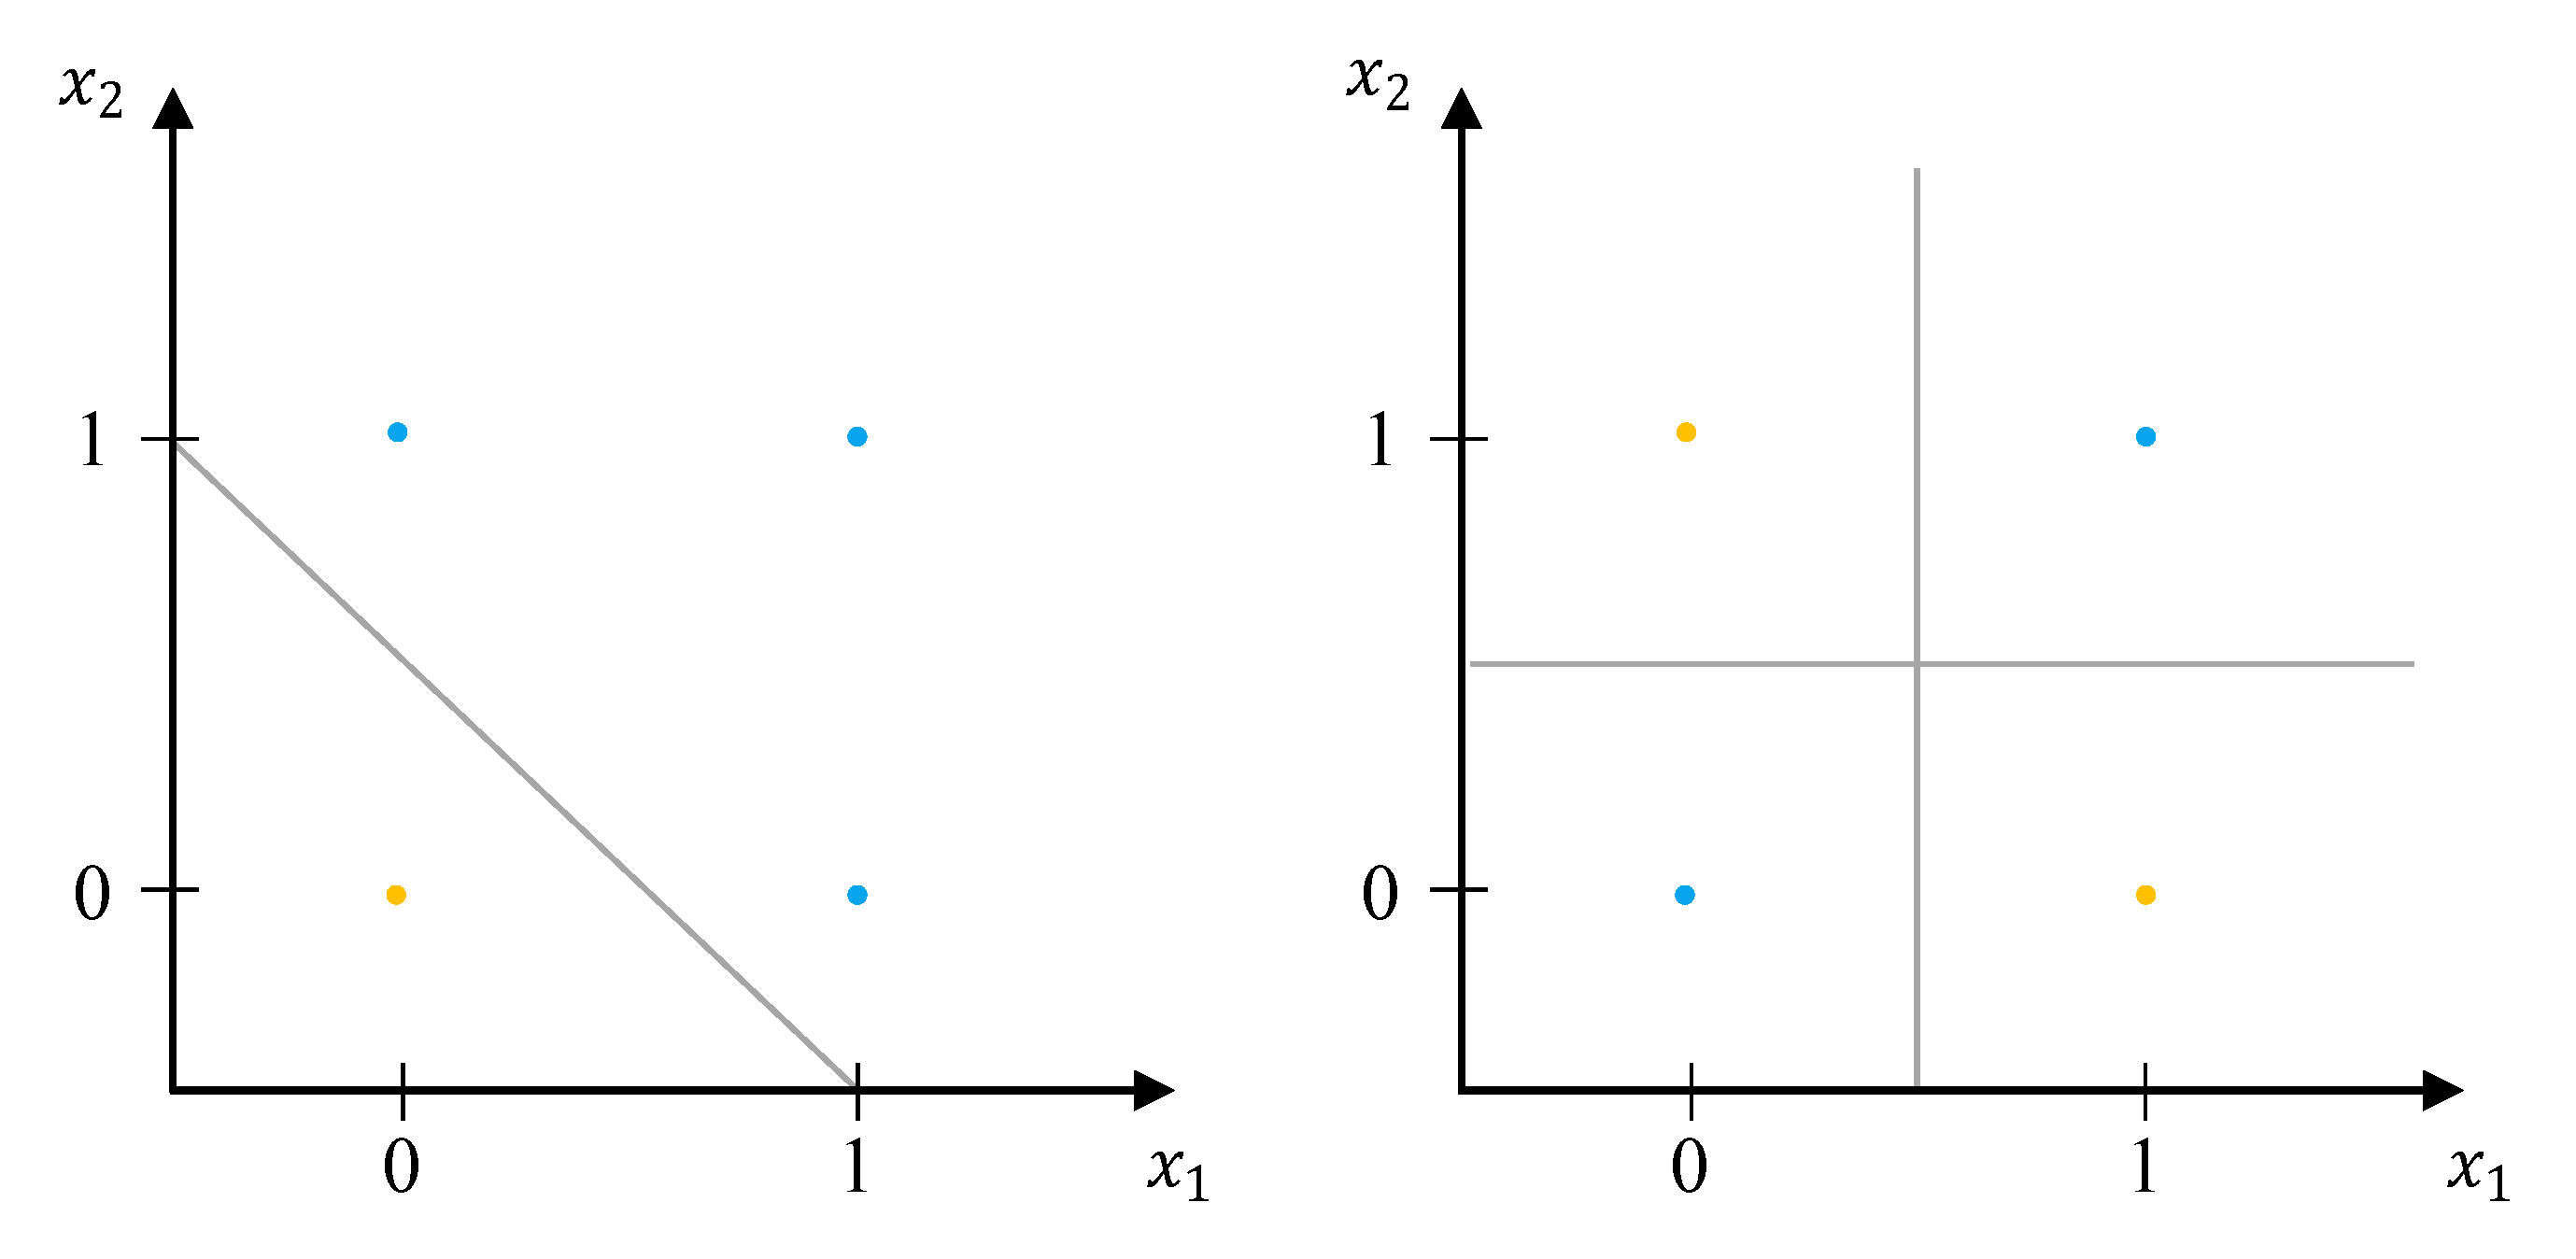
\includegraphics[width=.9\linewidth]{images/xor}
    \caption[Limits of the linear model.]{While linear models can learn decision boundaries for \textit{linear separable} data, e.g.\ learning the \textit{logical or}-function (left), they are incapable of learning non-linear decision boundaries, e.g.\ the \textit{XOR}-function (right)~\autocite{sonnet2022NeuralBoook}.}
    \label{fig:xor}
\end{figure}
As seen in \autoref{fig:xor}, linear models can only learn linear \textit{decision boundaries}.

In the 1980s, the movement of \enquote{connectionism} improved upon these initial approaches.
The main idea of this movement is that a large number of simple computational units (i.e.\ neurons) can realize intelligent behaviour when working together.
With this idea in mind, a possible solution for the XOR-problem is given by feeding the input in two independent linear models and combining their outputs in a third linear model.

More precisely, the inputs $\boldsymbol{x} = [x_1,x_2]$ are initially mapped to an intermediate state often referred to as \enquote{hidden units}.
\begin{align*}
    f^{(1)}(\boldsymbol{x}; \boldsymbol{w_1}, b_1) = g(\boldsymbol{w_1}^T \boldsymbol{x} + b_{1}) = z_1 \\
    f^{(2)}(\boldsymbol{x}; \boldsymbol{w_2}, b_2) = g(\boldsymbol{w_2}^T \boldsymbol{x} + b_{2}) = z_2
\end{align*}
Because the composition of multiple linear functions would just collapse into another linear function, a non-linear \textit{activation function} $g$ is applied.
A function that is commonly used is the \textit{rectified linear unit} or \textit{ReLU} defined as $g(v) = \max\{0, v\}$.
The hidden units are then passed to the third linear model which produces the final output:
\[
    f^{(3)}(\boldsymbol{z} = [z_1, z_2]; \boldsymbol{w_3}, b_3) = \boldsymbol{w_3}^T \boldsymbol{z} + b_{3} = y
\]
The function $f^{(1)}$ and $f^{(2)}$ can be combined into a single function $f^{\{1, 2\}}$ parameterized by a weight matrix $\boldsymbol{W}$ and a bias vector $\boldsymbol{b}$:
\[
    f^{\{1, 2\}}(\boldsymbol{x}; \boldsymbol{W}, \boldsymbol{b}) = g(\boldsymbol{W}^T \boldsymbol{x}+ \boldsymbol{b}) = \boldsymbol{z} \\
\]
The non-linear function $g$ is applied component wise.
The complete network can now be written as a simple composition of functions:
\[
f(\boldsymbol{x}) = f^{(3)}(f^{\{1, 2\}}(\boldsymbol{x}))
\]
$f^{(1)}$, $f^{(2)}$ and $f^{(3)}$ are called the \enquote{neurons} of the network.
Multiple neurons that can be computed in parallel are called a layer.
In this case $f^{\{1, 2\}}$ is called a \enquote{hidden layer}, the inputs $\boldsymbol{x}$ are the \enquote{input layer} and $y$ is the \enquote{output layer}.

With this simple neural network, it is indeed possible to learn the XOR-function.
Furthermore, this method can be modified to find functions that can approximate almost any possible function.
The \textit{universal approximation theorem} states, that a network with a linear output layer and a hidden layer with an appropriate non-linear activation function can represent any Borel measurable function that maps from one finite-dimensional space to another, as long as there are enough hidden units~\autocite{Goodfellow-et-al-2016}.
In practice, it is not feasible to use such a single layer network because the number of necessary hidden units grows exponentially for more complex functions.
Instead, it is common to add more hidden layers by chaining more functions:
\[
    f(\boldsymbol{x}) = f^{(4)}(f^{(3)}(f^{(2)}(f^{(1)}(\boldsymbol{x}))))
\]
The number of hidden layers is called the \enquote{depth} of the network.
The depth is also what the term \enquote{deep learning} refers to.
It is not exactly defined what number of layers a neural network needs to be called \textit{deep}.
But a \acrlong{dnn} can be generally understood as a neural network with many layers.

The previously described neural network is known as a \enquote{feedforward neural network} or \gls{mlp}.
It can be easily scaled by adding any number of layers with any number of neurons.
A typical way of visualizing a \gls{mlp} can be seen in \autoref{fig:neural-network}.
\begin{figure}
    \centering
    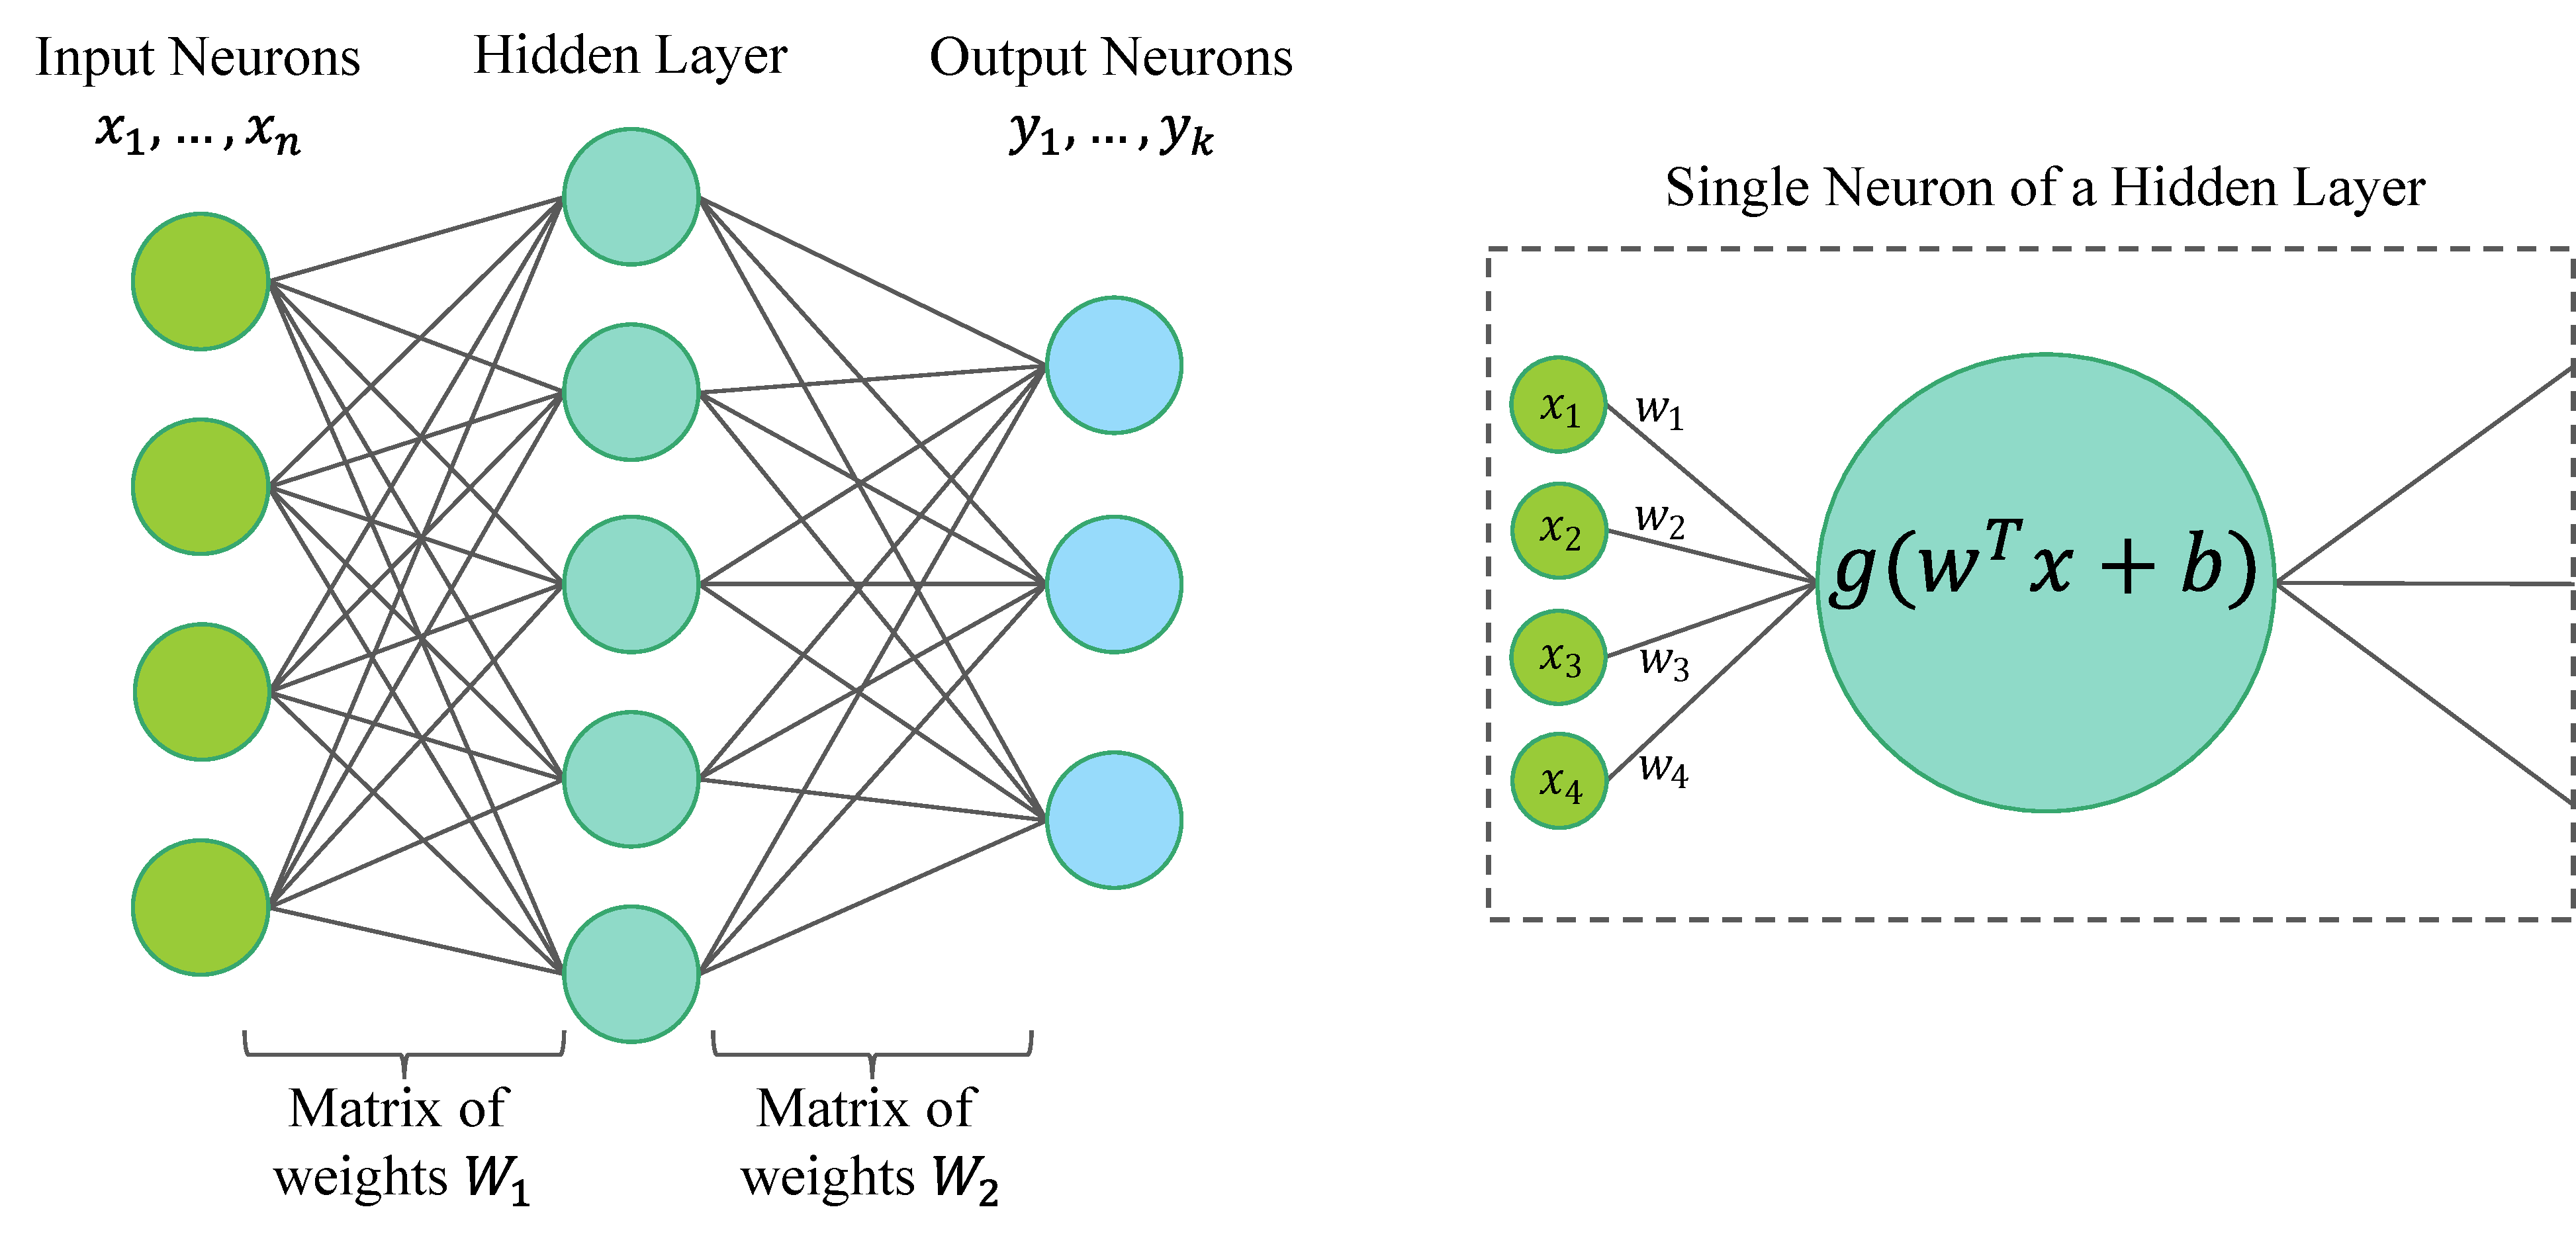
\includegraphics[width=\linewidth]{images/nn}
    \caption[Visualization of a neural network.]{Neural networks are often visualized as directed graphs. This \gls{mlp} (left) has four input neurons, one hidden layer with five neurons and three output neurons. Each hidden unit or neuron is represented by a node. The edges between neurons stand for the weights that are applied to the incoming signals. The edges between two layers are mathematically described by a single matrix $\boldsymbol{W}$ that multiplied with the previous outputs gives the inputs for the next layer~\autocite{sonnet2022NeuralBoook, Goodfellow-et-al-2016}.}
    \label{fig:neural-network}
\end{figure}
% \enquote{feedforward} because information flows only in one direction

\glspl{dnn} like the \gls{mlp} have been successfully applied to many tasks like \textit{speech recognition}, \textit{image segmentation} and \textit{optical character recognition}.
They incorporate little task-specific assumptions and are thus a very general approach.
The design of \glspl{mlp} makes it possible to choose input and output dimensions freely to describe any supervised learning task.
\glspl{mlp} handle high dimensional data (e.g.\ images) well.
This is related to the ability of \glspl{dnn} to learn features automatically from raw input data.
In traditional \gls{ml}-applications the features that were passed to the model as inputs were often selected by hand.
The raw input data was processed, so only information relevant to the task remained.
This is known as \textit{Feature Engineering}.
Depending on the complexity of the task and data, a lot of manual effort is needed to find effective features.
Having the model learn the features automatically is called \enquote{feature learning} or \enquote{representation learning}.
The concept of \textit{representations} is crucial in deep learning.

%often better than hand selected features

% \gls{dnn} generates different representation at each layer
% specific layers react or activate for specific features
% Intution of learning different things in each layer
% highlighting different parts of input, ephasizing

% earlier layers output representations that make later task easier e.g. classification
% -> example XOR linear separability -> hidden layer maps into a different feature space

%often better than hand selected features
% during supervised training rich representations are learned
% reusablility of parts of network

% whole field of research dedicated to finding general purpose representation

\glspl{dnn}



% - representation learning

%\enquote{respresentation learning} -> not only mapping but also learning features
%
%factors of variation make learning difficult (e.g. recognizing a car in an image -> different angles)
%
%each mathematical function outputs new representation of input
%
%more available data -> Deep Learning more useful
%overfitting no issue

%nesting of concepts in layers of network

%concept of distributed representation:
%3 subjects, 3 colors -> model should recognize all 9 combinations
%possible with 9 neurons that each learn to identify one combination
%better: 3 neurons describe color and 3 the type of object (concatenation? intermediate representation)
%
%1990s: advances in Sequence modeling -> LSTM
%

\subsubsection{Training Neural Networks}
Neural networks are usually trained by applying some form of gradient descent.

- Backpropagation
% Training dificult: inductive biases
% \enquote{incorporate doamin knowledge into the network} -> cnn, parameter sharing -> reduce trainable parameters while having equal size

% modern models designed  to have nice properties for optimization (LSTM) (seite 341)
% skip connection
% cnn: sprase interaction
% less calculations

%from~\autocite{sonnet2022NeuralBoook}:
%The term \enquote{Deep Learning} was first used in book in 2000

% MLPs have not been widely used in pratice: goodfellow and bias paper


\subsubsection{Loss Functions / Example Classification}


\section{Transformers}\label{sec:trans}


\section{Decoder-only Models}\label{sec:decoder}

\subsection{GPT}\label{subsec:gpt}

\subsection{Llama}\label{subsec:llama}

\subsubsection{Leo}


\section{Supervised Fine-Tuning (SFT)}\label{sec:supervised-fine-tuning}


\section{Alignment Methods}\label{sec:alignment-methods}
from~\autocite{zhao2023survey}:
capture properties of training corpus

\subsection{RLHF}\label{subsec:rlhf}

\subsection{PPO}\label{subsec:ppo}

\subsection{DPO}\label{subsec:dpo}
